Con este título tan críptico quería hacer referencia al formato del
texto. Hasta ahora hemos escrito cosas pero nos hemos conformado con el
que nos aparece por defecto, hoy vamos a aprender a cambiar el tamaño y
estilo de la letra y a escribir en diferentes colores. Pero para ello
antes de nada tenemos que entender qué es una clase y cómo afecta a
nuestro documento.

\section{Clases}\label{sec:clases}

Lo primero que tenemos que saber es que el formato de nuestro documento
está definido por su clase. Ahí pondrá cómo de grande tienen que ser los
títulos, cuánto espacio tiene que haber entre los ítems de una lista o
el tamaño de los márgenes. Estas clases pueden ser las típicas
\lstinline!article! o \lstinline!book!, unas que vivan en un paquete
como las \href{http://www.ctan.org/pkg/tufte-latex}{clases Tufte} o
incluso unas que hayamos escrito nosotros mismos. Son simplemente un
archivo \emph{cls} lleno de definiciones.

La clase del documento la establecemos en la definición inicial:

\begin{lstlisting}[language={[latex]tex}]
% Usar la clase memoir
\documentclass{memoir}
\end{lstlisting}

Ahora que sabemos que el estilo de nuestro documento lo decide la clase,
vamos a ver cómo cambiar alguna cosa puntual en el documento. Digo
puntual porque si queremos, por ejemplo, que todos los títulos de
sección sean en cursiva es preferible que redefinamos la orden en
cuestión. Ya haremos eso en el futuro, no os preocupéis.

\section{Formato de texto}\label{sec:formato}

Empecemos modificando el texto. Vamos a cambiar su tamaño, le
aplicaremos diferentes estilos y, por último, haremos una pequeña
introducción al color en LaTeX.

\subsection{Tamaño}\label{sec:tamano}

La manera en la que LaTeX trata el tamaño de letra es bastante original:
coge como referencia el tamaño de la letra del cuerpo del documento y
define los demás tamaños de manera relativa respecto a este. Así, si
cambiamos el tamaño de letra del cuerpo todo lo demás cambia en
consonancia.

Recordemos que el tamaño de letra del cuerpo lo podemos establecer como
argumento opcional en \lstinline!\documentclass!:

\begin{lstlisting}[language={[latex]tex}]
\documentclass[11pt]{article}
\end{lstlisting}

Si no ponemos nada, usará
\href{http://tex.stackexchange.com/questions/155896/what-is-the-default-font-size-of-a-latex-document\#155899}{10pt}
por defecto.

En esta tabla del libro sobre
\href{https://en.wikibooks.org/wiki/LaTeX/Fonts\#Sizing_text}{LaTeX en
Wikibooks} están los comandos para agrandar y reducir la letra y su
respectivos tamaños de letra según el tipo de documento que estemos
creando. Tanto \lstinline!article! como \lstinline!book! son parte de
las
\href{http://tex.loria.fr/ctan-doc/macros/latex/doc/html/usrguide/node10.html}{clases
estándar}.

\begin{figure}[htbp]
\centering
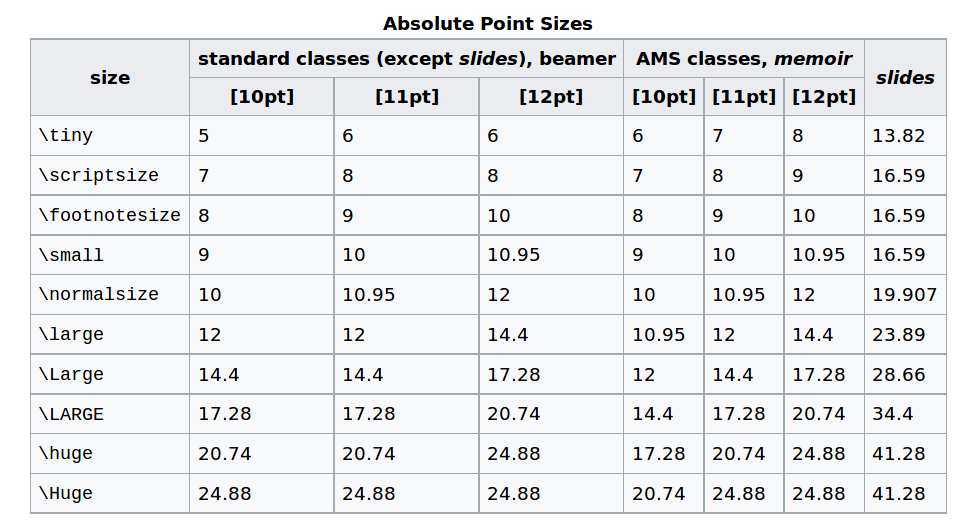
\includegraphics[width=0.9\textwidth]{docs/Figuras/tamanoLetra.png}
\end{figure}

Para usar cualquiera de estos comandos hay dos opciones, usarlos dentro
de una línea o como entorno. Si los usamos en la propia línea, harán
efecto hasta el final del \emph{grupo} (una zona delimitada entre
llaves) o \emph{entorno} actual. Si la zona de aplicación no está
delimitada, el tamaño de letra se mantendrá hasta encontrarse con otro
comando de tamaño o hasta el final del documento. Veamos un ejemplo para
entenderlo mejor:

\begin{lstlisting}[language={[latex]tex}]
Texto normal {\Huge Texto gigantesco}

\normalsize Texto normal hasta nueva orden

\section{\Huge Título de sección enorme}

Texto normal

\begin{quote}
  \Large Letra grande solo para la cita
\end{quote}

Texto normal de nuevo

\small Texto pequeño hasta el final del documento
\end{lstlisting}

Si el trozo de texto que queremos personalizar es muy largo, tal vez
merezca la pena usar el entorno para ganar en legibilidad:

\begin{lstlisting}[language={[latex]tex}]
\begin{tiny}
    Miniletrilla 
\end{tiny}
\end{lstlisting}

También podemos establecer otros tamaños de letra como haríamos en los
editores de toda la vida. Para ello utilizamos el comando
\lstinline!\fontsize!:

\begin{lstlisting}[language={[latex]tex}]
\fontsize{tamaño}{baseline skip}\selectfont Texto
\end{lstlisting}

Podemos facilitar ambos argumentos en diferentes unidades, si no ponemos
más que el número, LaTeX entenderá que estamos hablando de
\emph{puntos}. El segundo argumento es importante, ya que fija la
distancia
\href{http://noodle.med.yale.edu/latex/latex2e-html/baselineskip.html}{\lstinline!\\baselineskip!},
es decir, la distancia entre las partes inferiores de dos líneas
sucesivas. Suele ser 1.2 veces el tamaño de fuente\footnote{He de decir
  también que ponernos a cambiar estas cosas sin dominar es el camino
  directo al infierno del LaTeX en el que todo queda mal y arreglamos
  una cosa y se rompe otra y no sabemos por qué.}.

Si utilizamos este sistema es preferible que usemos una \emph{fuente
vectorial}, así estará disponible en cualquier tamaño\footnote{Para una
  explicación mejor sobre los tipos de fuente podéis echarle un ojo al
  artículo de la
  \href{https://en.wikipedia.org/wiki/Computer_font}{Wikipedia}.}. Por
ejemplo, con Computer Modern es probable que nos salga un aviso de este
estilo:

\begin{lstlisting}[language={[latex]tex}]
LaTeX Font Warning: Font shape `OT1/cmr/m/n' in size <20> not available
(Font)              size <20.74> substituted on input line 25.
\end{lstlisting}

Esto ocurre porque la fuente
\href{https://en.wikipedia.org/wiki/Computer_Modern}{Computer Modern} es
del tipo
\href{https://en.wikipedia.org/wiki/Computer_font\#Bitmap_fonts}{\emph{bitmap}},
es decir, las letras están formadas por puntitos. Esto implica que hay
versiones de la fuente para tamaños concretos, no para todos. En este
caso, lo más fácil es pasarnos a
\href{http://www.gust.org.pl/projects/e-foundry/latin-modern}{Latin
Modern} (\lstinline!\usepackage{lmodern}!) que es igualita y como es
\href{https://es.wikipedia.org/wiki/OpenType}{OpenType} (y por lo tanto
vectorial) no tiene este problema. Además es compatible con la
codificación T1, algo que necesitamos
\href{https://ondahostil.wordpress.com/2017/02/21/curso-no-convencional-de-latex-a-vueltas-con-el-idioma/}{si
vamos a escribir acentos}.

\subsection{Forma}\label{sec:forma}

De momento en el tema de las formas vamos a ignorar el tipo de fuente y
vamos a hablar de negritas, cursivas y esas cosas. Sobre el tipo de
fuente hablaremos en el futuro, que
\href{https://ondahostil.wordpress.com/2016/12/03/lo-que-he-aprendido-escribir-una-carta-en-latex/}{da
para rato}.

Una cosa que aprendí yo hace poquito es que en LaTeX el estilo de cada
letra pertenece a una \emph{familia}, una \emph{serie} y una
\emph{forma}:

\begin{itemize}
\itemsep1pt\parskip0pt\parsep0pt
\item
  La familia indica cómo es la fuente: con serifas o \emph{roman}
  (\lstinline!\rmfamily!), sin serifas (\lstinline!\sffamily!) o
  monoespaciada (\lstinline!\ttfamily!)
\item
  La serie hace referencia al grosor del trazo: fino
  (\lstinline!\lfseries!), medio (\lstinline!\mdseries!) o grueso
  (\lstinline!\bfseries!)
\item
  La formas como su nombre indica describen la forma de las letras:
  recta (\lstinline!\upshape!), cursiva
  (\lstinline!\itshape), oblicua (!\slshape`) o
    versalita (`\scshape`).
\end{itemize}

La letra por defecto tiene serifas, es de grueso medio y recta, es a lo
LaTeX denomina \lstinline!\normalfont!. Podemos hacer otras
combinaciones siempre con un elemento de cada grupo. Saber esto es
especialmente útil cuando estamos definiendo nuestro propio estilo.

Podemos activar diferentes familias, series y formas con diferentes
comandos{[}\^{}comand{]}:

\begin{itemize}
\itemsep1pt\parskip0pt\parsep0pt
\item
  \lstinline!\textbf{}! pone el texto en negrita
\item
  \lstinline!\textit{}! sirve para activar la cursiva
\item
  \lstinline!\texttt{}! escribe en letra de máquina de escribir o
  monoespaciada
\item
  \lstinline!\textsc{}! para las versalitas
\item
  \lstinline!\textnormal{}! vuelve a \lstinline!\normalfont!
\end{itemize}

Hay claramente un patrón, ¿verdad?

Podemos anidar estos comandos y escribir en letra monospaciada, cursiva
y negrita simultáneamente si nos parece que es una buena idea. En
cualquier caso, este es un tema complejo y esto no deja de ser una
explicación un poco por encima, en las referencias podéis encontrar más
información.

Como veis, no aparece la opción de subrayar porque es una
\href{http://practicaltypography.com/underlining.html}{muy mala decisión
tipográfica} que proviene de los tiempos en los que se escribía a
máquina. Si aun así queréis subrayar porque sois tercos como mulas, lo
que estáis buscando es el comando \lstinline!\underline{}!. También
tenéis el paquete \href{http://www.ctan.org/pkg/ulem}{\lstinline!ulem!},
que proporciona el comando \lstinline!\ul! para subrayar y del que me
niego a hablar.

Una cosa interesante es el comando \lstinline!\emph{}! que sirve para
enfatizar. En general se comporta como la cursiva aunque con un par de
pequeñas diferencias:

\begin{itemize}
\itemsep1pt\parskip0pt\parsep0pt
\item
  Depende del contexto, por ejemplo, si enfatizamos un trozo que estaba
  ya en cursiva se pone recto:
\end{itemize}

\begin{lstlisting}[language={[latex]tex}]
\textit{Texto en cursiva \emph{texto recto}}
\emph{Texto en cursiva \emph{texto recto}} 
\end{lstlisting}

\begin{itemize}
\itemsep1pt\parskip0pt\parsep0pt
\item
  Podemos modificarlo para enfatizar a nuestro gusto, ya sea en negrita,
  con colores o lo que sea. Es precisamente lo que hace el paquete
  \lstinline!ulem! (\emph{underline emphasis})
\end{itemize}

\subsection{Color}\label{sec:color}

¡Por fin llegamos al color! Tenía ganas ya, es cansino todo en blanco y
negro. Como suele ser habitual, para usar colores en LaTeX necesitamos
un paquete: \href{http://www.ctan.org/pkg/xcolor}{\lstinline!xcolor!},
la evolución del paquete
\href{https://www.ctan.org/pkg/color}{\lstinline!color!}. Lo cargamos en
el preámbulo con unas pocas opciones que nos facilitan la vida:

\begin{lstlisting}[language={[latex]tex}]
\usepackage[usenames,dvipsnames,svgnames,table]{xcolor}
\end{lstlisting}

\begin{itemize}
\item
  \lstinline!usenames! permite que llamemos a los 16 colores básicos por
  su nombre en lugar de por su definición
\item
  \lstinline!dvipsnames! nos da acceso a otros 64 colores extra
\item
  \lstinline!svgnames! añade otros 150 colores más
\item
  \lstinline!table! nos deja usar colores en las tablas
\end{itemize}

Tenéis una explicación sobre los colores disponibles en el apartado
\href{http://osl.ugr.es/CTAN/macros/latex/contrib/xcolor/xcolor.pdf}{2.4
del manual de \lstinline!xcolor!}.

Para cambiar el color del texto podemos usar tanto
\lstinline!\textcolor! como \lstinline!\color!:

\begin{lstlisting}[language={[latex]tex}]
\textcolor{red}{texto de color rojo}

{\color{magenta} texto en color rosa raro}
\end{lstlisting}

Al igual que ocurría con los comandos para cambiar el tamaño de letra,
en este caso \lstinline!color! afecta hasta el final del grupo.

También podemos definir nuestros propios colores con
\lstinline!\definecolor! dándoles un nombre o directamente cuando los
vayamos a usar. Para ello necesitamos elegir un modelo de color (rgb,
cmyk, HTML, \ldots{}) y darle el valor correspondiente:

\begin{lstlisting}[language={[latex]tex}]
% RGB
\definecolor{azulito}{rgb}{0.36, 0.54, 0.66}

% HTML (en hexadecimal y mayúsculas)
\definecolor{otroColor}{HTML}{4070A0}

% Definir directamente al usarlo
{\color[HTML]{4070A0} texto en color}
\end{lstlisting}

Definir nuestros propios colores es especialmente útil cuando queremos
combinar los colores del texto con alguno específico de una imagen o si
las opciones \lstinline!dvipsnames! y \lstinline!svgnames! no nos
funcionan por algún motivo. En la página
\href{http://latexcolor.com/}{\emph{LaTeX color}} hay montones de
definiciones de colores para que empecemos a jugar.

\section{El resumen}\label{sec:resumen7}

Vamos a hacer una recapitulación sobre lo que hemos visto hoy, que es
largo y denso:

\begin{itemize}
\item
  \textbf{Tamaño}: los tamaños en LaTeX son relativos y se cambian con
  comandos que van de \lstinline!\tiny! para la letra más pequeña a
  \lstinline!\Huge! para la más grande. También se puede establecer un
  tamaño de fuente concreto, pero con cuidado.
\item
  \textbf{Forma}: los estilos de las letras se dividen en familias,
  series y formas que pueden combinarse entre sí. A cada elemento le
  corresponde un comando que activa un formato específico. El texto por
  defecto tiene serifas, es de grueso medio y recto, se conoce como
  \lstinline!\normalfont!.
\item
  \textbf{Color}: para usar colores en LaTeX necesitamos el paquete
  \lstinline!xcolor!. Sus diferentes opciones nos dan acceso a un número
  de colores predefinidos pero también existe la posibilidad de definir
  unos nosotros con \lstinline!\definecolor{modelo}{definición}!.
  Aplicamos al texto cualquiera de estos colores con
  \lstinline!\textcolor{color}{texto}! o con \lstinline!\color{color}!.
\end{itemize}

\section{Referencias}\label{sec:referencias7}

\href{http://texcatalogue.ctan.org/bytopic.html\#classes}{\emph{Classes}
en \emph{The TeX catalogue}}

\href{http://tex.stackexchange.com/questions/782/what-are-the-available-documentclass-types-and-their-uses}{\emph{What
are the available ``documentclass'' types and their uses?} en
StackExchange}

\href{http://www.ctan.org/pkg/tufte-latex}{\emph{Tufte-LaTeX} en CTAN}

\href{https://www.sharelatex.com/learn/Line_breaks_and_blank_spaces}{\emph{Line
breaks and blank spaces}}

\href{http://tex.stackexchange.com/questions/74353/what-commands-are-there-for-horizontal-spacing\#74354}{\emph{What
commands are there for horizontal spacing?} en TexExchange}

\href{https://en.wikibooks.org/wiki/LaTeX/Fonts}{\emph{LaTeX/Fonts} en
Wikibooks}

\href{https://www.sharelatex.com/learn/Font_sizes,_families,_and_styles}{\emph{Font
sizes, families, and styles}}

\href{https://www.tug.org/pracjourn/2006-1/schmidt/schmidt.pdf}{\emph{Font
selection in LaTeX: The most frequently asked questions} (pdf)}

\href{http://www.cl.cam.ac.uk/\%7Erf10/pstex/latexcommands.htm}{\emph{LaTeX
font commands}}

\href{https://github.com/wspr/fontspec}{\emph{The \lstinline!fontspec!
package}}

\href{https://en.wikibooks.org/wiki/LaTeX/Page_Layout\#Margins}{\emph{LaTeX/Page
Layout} en WikiBooks}
